\documentclass[11pt]{article}
\usepackage{fullpage,graphicx,float,amsmath,enumitem,hyperref}
\setlist{parsep=5.5pt}
\setlength{\parindent}{0pt}
\setlength{\parskip}{\baselineskip}

\usepackage{fancyhdr}
\pagestyle{fancy}
\lhead{Missing Data and LOD}
\rhead{Paul Harmon, Nnamdi Ezike, and Andrea Mack}
\setlength{\headheight}{18pt}
\setlength{\headsep}{2pt}

\title{Pea Lodging Final Report}
\author{Client: Jamin Smitchger\\
Consultants: Paul Harmon, Nnamdi Ezike, and Andrea Mack}
\date{December 16, 2016}

\begin{document}
\maketitle





\section{Introduction}
Jamin is a Ph.D. student in the Department of Plant Sciences and Plant Pathology at MSU. The primary focus is his research is to associate variation in genetic expression with variation in the expression of several phenotypic traits. Genotypic and pheynotypic data were collected on 257 varieties of pea, from two locations (Bozeman and Moccasin), over 4 years. Phenotypic data includes percent lodging, tendril length, tendril node length, nodes at 1st flow, maximum number of nodes, germination, number of branches, plant height, plant length, average total yield, main stem diameter, tiller diameter, ``comp" tiller diameter, and maturation time, totaling 14 traits. Data from 609 genetic markers were collected. The end result of Jamin's research will include a quantitative trait loci (QTL) analysis. Prior to the QTL analysis, understanding of the data and methods are necessary. The report includes:

\begin{itemize}

\item Evaluation of correlations in pheynotypic data

\item Analysis of combining data from the different sites and years

\item Exploration of the rate of missing data

\item Explanation of significance thresholds for QTL 

\item Suggestions for future work
\end{itemize}
\pagebreak

\section{Correlation Plots}
Correlation describes the strength and direction of a linear association. Specifically, this analysis examines Pearson Correlations because the variables are measured on a quantitative scale.  Correlation is measured on a scale between -1 (a perfect negative linear association) and 1 (a perfect positive linear association). Correlation does not imply causal relationships. In examining, for instance, the relationship between lodging and stem width, the Pearson Correlation would only give information about the linear association between the two variables.  A strong association between the two variables cannot be interpreted that changes in stem width cause changes in lodging; rather, we would simply say that the two variables are associated with each other. Other confounding variables, such as climate, may be driving both. Since the phenotypes in each year at each site are considered separate response values, we consider examining plots of correlation matrices for each site/year combination as well as for the entire dataset. This allows for direct examination of linear relationships between covariates; however, non-linear relationships may not be accurately measured by Pearson correlation. Further investigation of outlying values in the data may be necessary as Pearson correlations are sensitive to the presence of outliers in the data. 

\subsection{Sites and Years Combined}
The correlation between pairwise explanatory variables of the phenotypic data were assessed using the a pairwise correlation matrix. We assessed the pairwise correlations across sites for pairs of explanatory variables which were measured within these sitesin at least two different years.

In Moccasin, only four variables were observed to have been measured both in 2015 and 2016. Of these variables, the length and main stem diameter of the plants are moderately correlated (r=-0.55). Also, the main stem diameter and root diameter of the plants are moderately correlated (r=0.45).
\pagebreak
\subsection{Bozeman in All Years}
The pairwise correlation matrix below shows that germination which was measured in Bozeman for all 3 years has weak correlation against all the variables measured. Also results from Bozeman shows that tendril length node of the plant was moderately to strongly correlated with the average length and tendril length of the plant with correlation coefficients of 0.61 and 0.48 respectively. The branch number and tiller diameter of the plant were also moderately correlated (r = 0.47). The maturity time of the plant was strongly and moderately correlated with the maximum nodes (r=0.65) and nodes of 1st flow (r=0.48). In addition, a correlation coefficient of 0.81 was observed for nodes 1st flow and maximum nodes of the plants.
\label{"Figure 1: Correlation Plot of Bozeman (In All Years)"}
\begin{knitrout}\footnotesize
\definecolor{shadecolor}{rgb}{1, 1, 1}\color{fgcolor}

{\centering 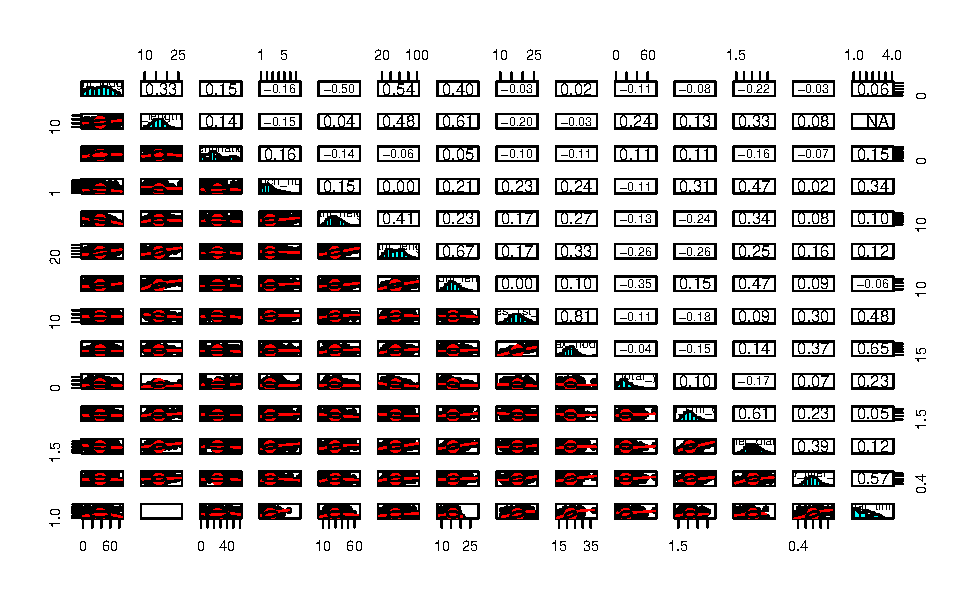
\includegraphics[width=\maxwidth]{figure/merged-1} 

}



\end{knitrout}




\subsection{Bozeman by Year}
We assessed the pairwise correlation of the different sites each year. In 2014, twelve pairs of explanatory variables had correlation coefficients between 0.42 and 0.91. The pairwise correlations are shown in the matrix below. Germination and total yield was strongly correlated (r=0.66) while the length and internode length of the plants recorded a very high correlation coefficient (r=0.91). In 2015 and 2016, of the pairwise combinations assessed, 28 combinations yielded correlation coefficients between 0.40 and 0.85. The results are presented in the pairwise correlation matrices below.

\begin{knitrout}\footnotesize
\definecolor{shadecolor}{rgb}{1, 1, 1}\color{fgcolor}

{\centering 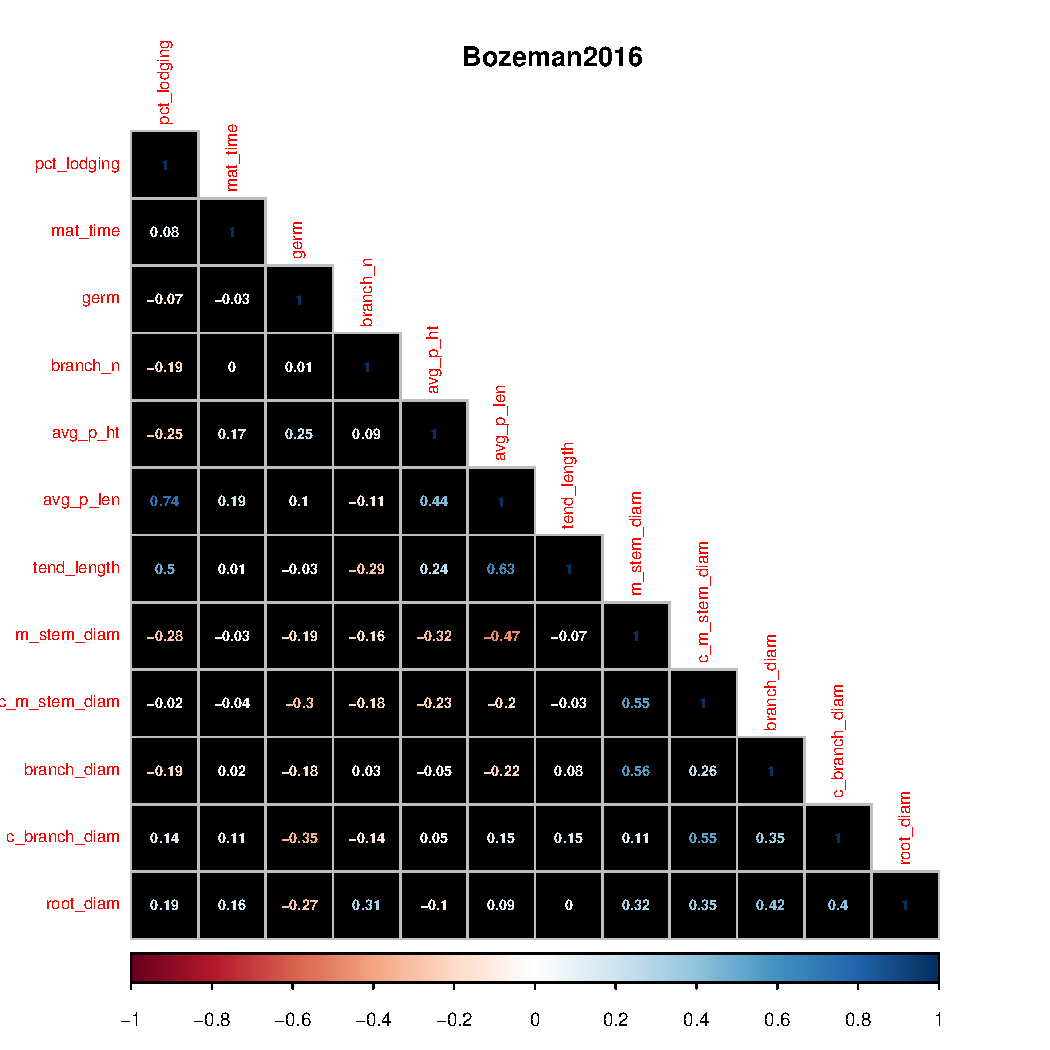
\includegraphics[width=\maxwidth]{figure/bz-1} 

}



\end{knitrout}

\begin{knitrout}\footnotesize
\definecolor{shadecolor}{rgb}{1, 1, 1}\color{fgcolor}

{\centering 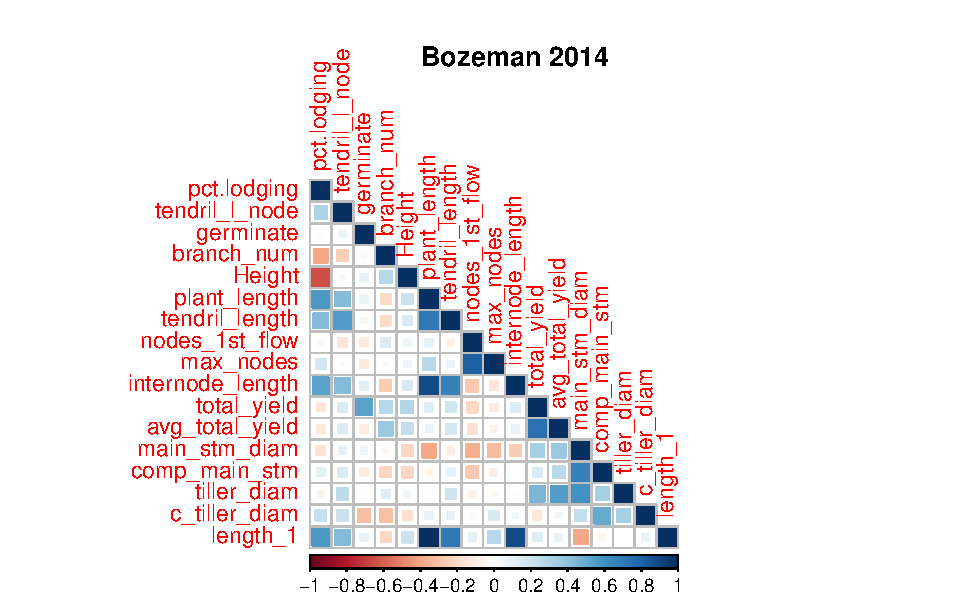
\includegraphics[width=\maxwidth]{figure/nextchunk-1} 

}




{\centering 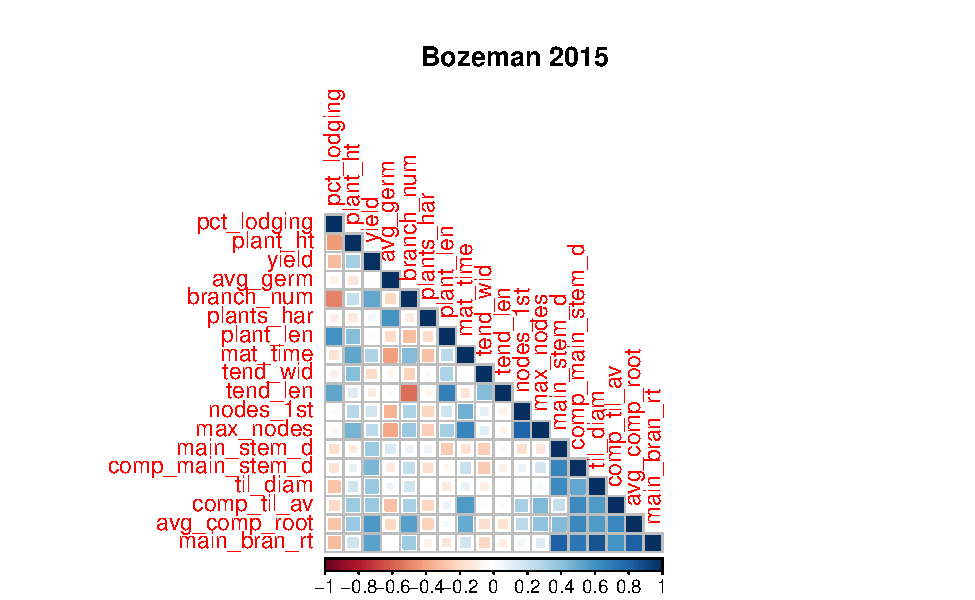
\includegraphics[width=\maxwidth]{figure/nextchunk-2} 

}



\end{knitrout}

\subsection{Moccasin by Year}
Examining the phenotypes at Moccasin in each year, we can see that several of the variables were relatively highly correlated in 2016. The strongest correlations were between tendril length and plant length, which makes sense, as well as between percent lodging and plant length. While none of the correlations would be interpreted as very strong, there are moderate postive and negative relationships in both years. 



\begin{knitrout}\footnotesize
\definecolor{shadecolor}{rgb}{1, 1, 1}\color{fgcolor}

{\centering 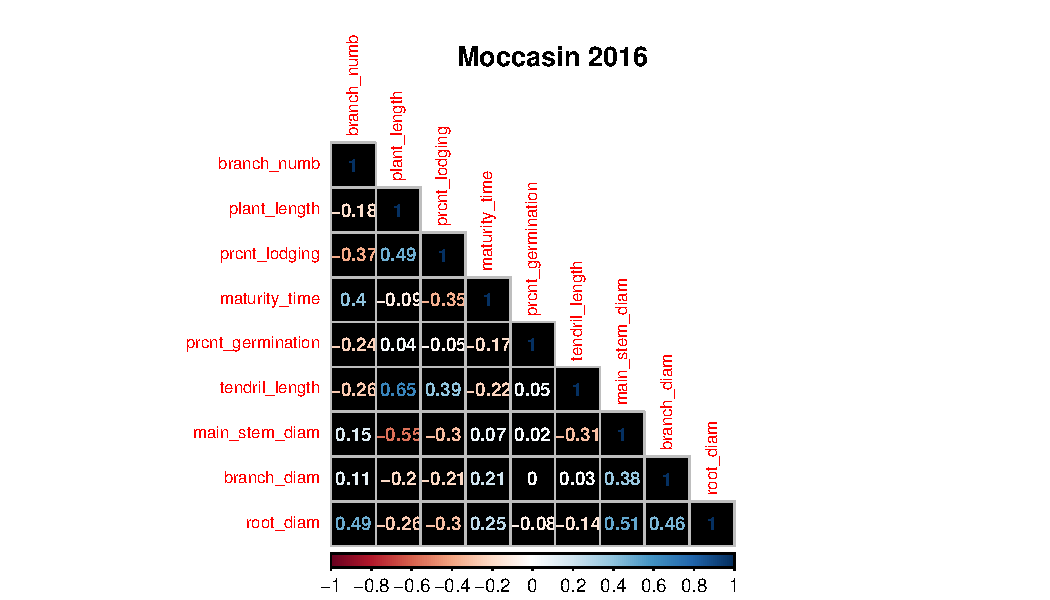
\includegraphics[width=\maxwidth]{figure/moc-1} 

}



\end{knitrout}
\pagebreak
In Moccasin in 2015, several notable correlations were found. Stress minus equation was strongly negatively correlated with tiller diameter, tiller compressed, tiller compressed flex, and flex after crushing. Lodging was found to be correlated with plant height as expected. 

\begin{knitrout}\footnotesize
\definecolor{shadecolor}{rgb}{1, 1, 1}\color{fgcolor}

{\centering 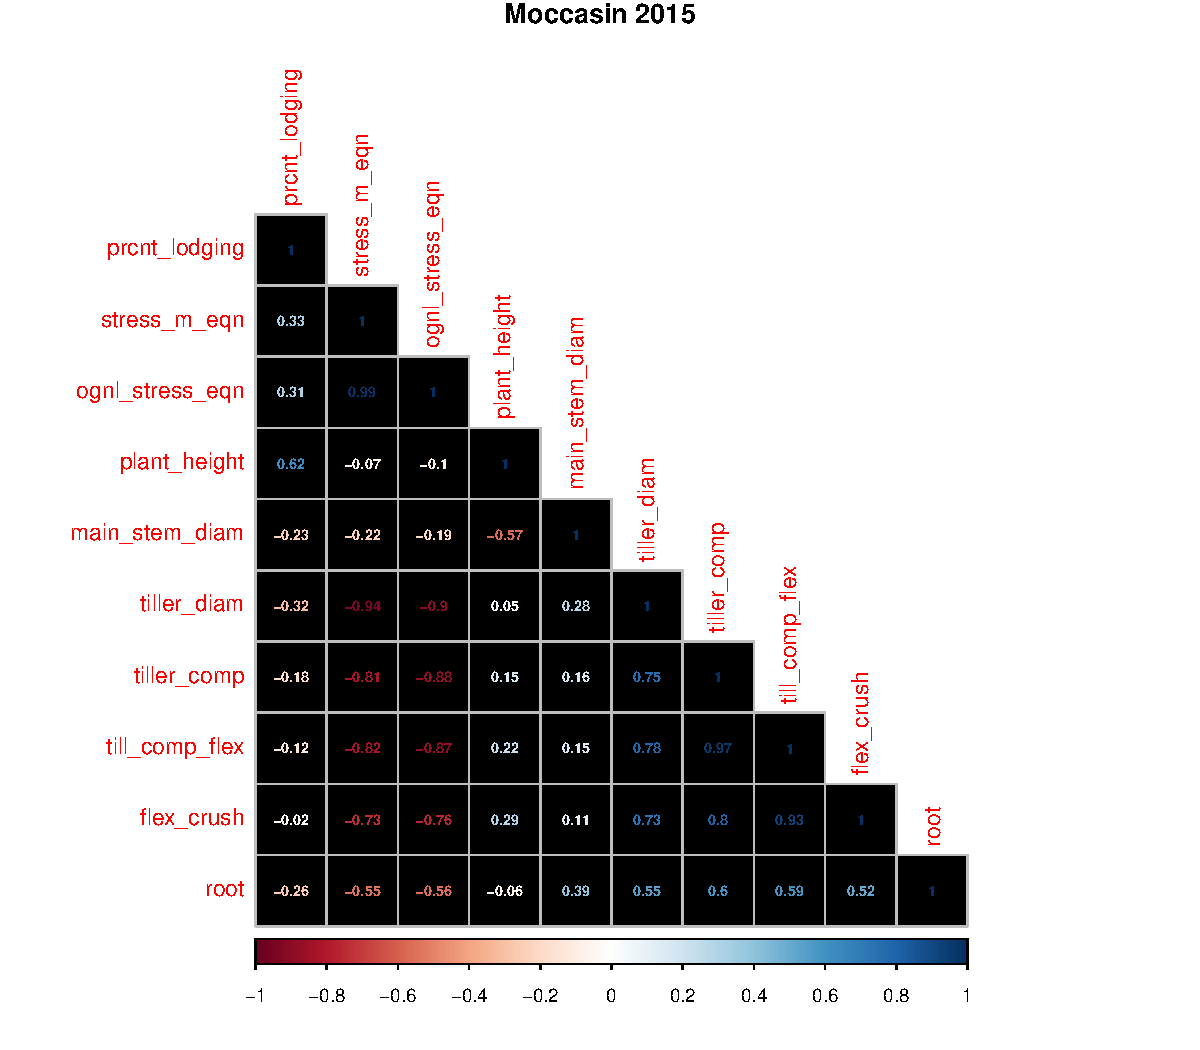
\includegraphics[width=\maxwidth]{figure/Moc15-1} 

}




{\centering 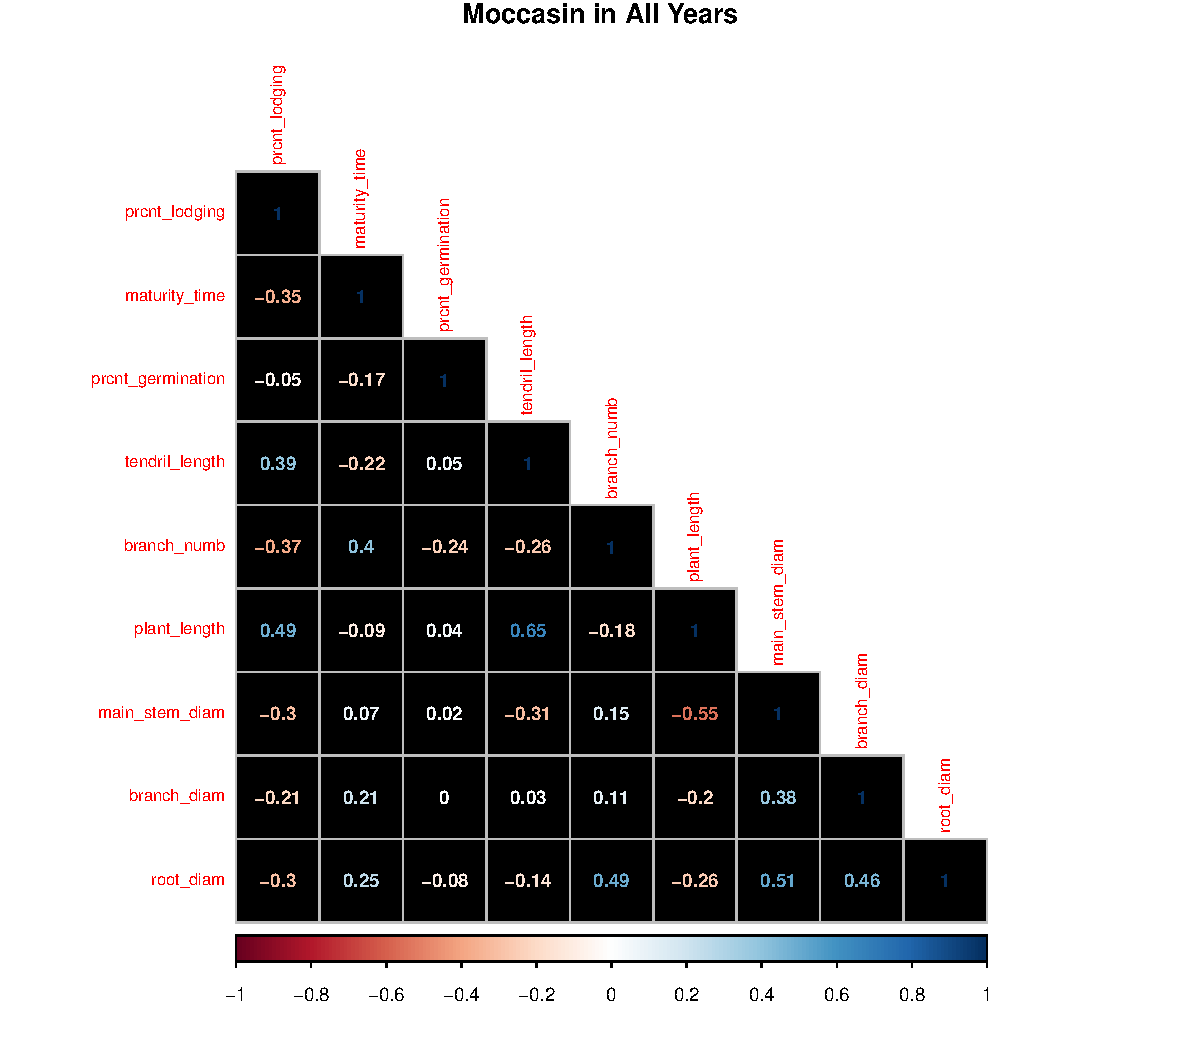
\includegraphics[width=\maxwidth]{figure/Moc15-2} 

}



\end{knitrout}
\pagebreak

\section{Site Year Combinations for Lodging}




\subsection{Exploratory Analysis} 
The data were collected over a period of 4 field seasons at sites in Bozeman and 2 field seasons in Moccasin. Phenotypic data were analyzed in order to determine whether conditions were similar enough at each year/site combination to consider as a single dataset, or if they differ by enough that the sites and years need to be considered as different groups.  

Though QTL analyses of all phenotypic traits is of interest, lodging is considered the primary response. Therefore, we examine the Percent Lodging measured at each site/year combination. Note that Percent Lodging is not measured in the 2013 Bozeman data; we did not include it in this analysis.

Visually, we can create beanplots (Kampstra 2008) to assess the differences mean percent lodging at each year/site combination.  These show both the variability of the distribution, like a traditional boxplot would, as well as information about the skew and modes. Over all years in Bozeman it appears that the distribution of lodging was slightly more variable than for sites in Moccasin; however, for some reason in 2016 the Bozeman site exhibited positive skew.  This indicates that in 2016, the majority of pea plants were lodged to a lesser degree than in 2015 or 2014.  The thin horizontal black bars indicate the original data values; the bold black lines indicate group means. 


\begin{knitrout}\footnotesize
\definecolor{shadecolor}{rgb}{1, 1, 1}\color{fgcolor}\begin{kframe}


{\ttfamily\noindent\bfseries\color{errorcolor}{Error in model.frame.default(formula = lodging \textasciitilde{} siteyear): variable lengths differ (found for 'siteyear')}}\end{kframe}
\end{knitrout}


\subsection{Interaction Plot}
If the sites are reasonably similar, we would expect to see parallel lines that are either overlapping or very near each other.  The dashed red line for Bozeman indicates that average percent lodging was higher in Bozeman than in Moccasin in both 2015 and 2016.  The bars indicate the variability of lodging for each year in Bozeman - it appears that for most years, Bozeman was slightly more variable than Moccasin. While the blue line and red line are both decreasing from 2015 to 2016, the difference in slopes indicates that there may be some interaction between year/site combinations.  This visualization indicates some evidence of a difference in lodging in each location and year. However, since there are no observations from Moccasin in 2014, we cannot formally test for a site by year interaction. 

\begin{knitrout}\footnotesize
\definecolor{shadecolor}{rgb}{1, 1, 1}\color{fgcolor}\begin{kframe}


{\ttfamily\noindent\bfseries\color{errorcolor}{Error in tapply(response, groups, fun): arguments must have same length}}\end{kframe}
\end{knitrout}

\pagebreak
\subsection{Regression Model and Pairwise Comparisons}
A model was fit to include all site and year combinations in order to test for differences between the combinations. Bozeman 2014 was treated as the baseline group. An overall F test using 4 and 1205 degrees of freedom to assess evidence against all site-year combinations yields a p-value less than 0.000001. There is strong evidence that the site/year combinations do not have all the same mean percent lodging. 
  
We include 95 percent confidence intervals for the true mean percent lodging at each site-year combination. In order to get a better sense for which groups differ, we performed Tukey-Kramer pairwise comparisons to adjust for multiple testing. The results of that analysis are included below. The plot below shows differing pairwise combinations were between Bozeman 2015 and Bozeman 2014, as well as between Moccasin 2015 and Bozeman 2016, and between Moccasin 2016 with Bozeman in 2015 and 2016. Given that Bozeman 2015 had such a large mean relative to the other site/year combinations, this is not a surprising result. 
  
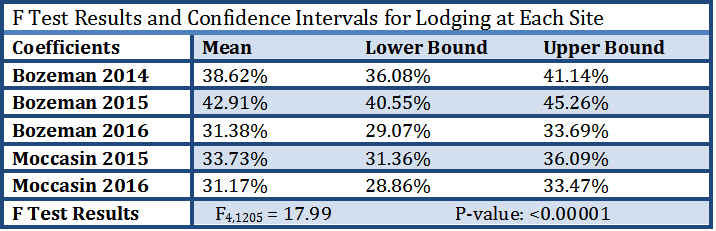
\includegraphics [width = 4.5 in] {RegressionResults}




























